Наиболее перспективным направлением развития исследованных в работе тем является применение адаптивных алгоритмов
к задачам группового обучения. Разработанный в работе алгоритм адаптивного подбора сложности пока применим 
только в постановках индивидуального обучения.
Для коллективного обучения такая модель слишком груба,поскольку не учитывает важные для образовательного 
коллектива процессы соревнования и
кооперации учащихся. Для аналитического описания группового обучения необходимо изучить три основных направления: \begin{enumerate}
    \item определение правил объединения в группы;
    \item подбор сложности задания для группы, учитывающий модель оценки эффективности совместной работы;
    \item оценка распределения нагрузки в случае группового задания.
\end{enumerate}

\begin{figure}[h]
    \centering
    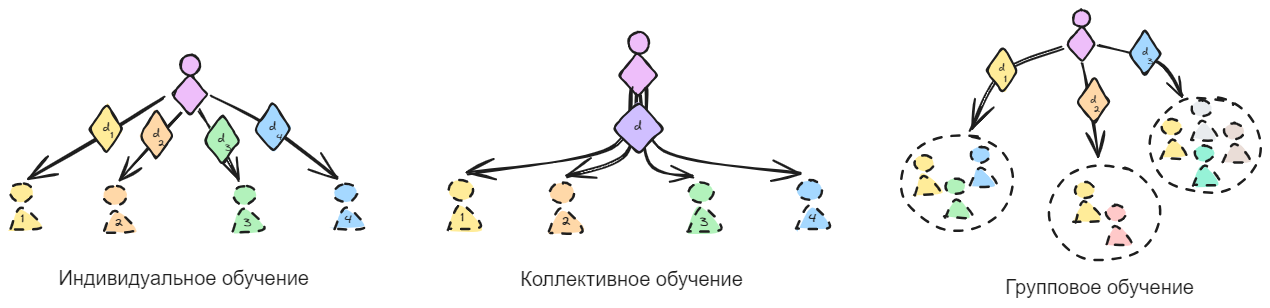
\includegraphics[width=0.95\textwidth]{assets/final/setting.excalidraw.png}
    \caption{Групповое обучение позволяет задать баланс между объемом проверки и специфичностью задания}
    \label{group_learning}
\end{figure}

При оценке экономической состоятельности корпоративного кодекса и культуры
венчурные фонды используют экономические модели организации \cite{marschak1972economic}
Теория охватывает широкий спектр проблем организации совместного труда. В частности, изучаются проблемы 
определения набора компетенций для членов команды \cite{radner1962team},
различия в целях между индивидом и коллективом \cite{groves1973incentives}\, 
тунеядства (от \textit{англ.} free-riders) и раскрытия корпоративной тайны \cite{francis2005disclosure}.
Разработанные модели также могут быть эффективно совмещены с 
алгоритмами распределения нагрузки \cite{kuhn1955hungarian} и дисконтирования вклада в будущем \cite{nash1950bargaining}.

Материал имеет потенциал для приложения к организации групповых проектов в образовании, поскольку
аналитически задает выводы о распределение нагрузки в коллективе. Моделирование выполняется 
путем введения совместной функции труда $Q(a_1,\dots,a_n)$, где $a_i$ соответствует вкладу $i$-ого участника.
Исследователи вводят разумные предположения о монотонности $\frac{\partial Q}{\partial a_i} > 0$ и порядке 
эффективности совместного вклада $\frac{\partial^2 Q}{\partial a_i^2} < 0$ и $\frac{\partial^2 Q}{\partial a_i \partial a_j} \ge 0$.
Таким образом, труд каждого участника дает вклад в результат, но стратегическое объединение имеет больший эффект. 

Изучение оптимального вклада каждого участника выполняется путем оптимизации целевой функции. 
Существуют различные подходы к её, но для задач
образования наиболее актуален баланс между усердиями учащихся и величиной приобретенных 
знаний $\sum_{i} \omega_i - g_i(a_i)$, где $\omega_i$ соответствует рейтинговому баллу
приобретенных знаний, а $g_i(a_i)$ --- задает монотонный отклик обучающегося $i$ на величину затраченного времени \cite{holmstrom1982moral}. Связь между трудом и баллами задается
организатором учебного процесса и, как правило, представляется как $\sum_{i} \omega_i = Q(a_1,\dots,a_n)$. Исследования позволят получить выводы об оптимальных нагрузках для учащихся
в случае логистического отклика. Таким образом, станет возможно аналитическое задание оптимального уровень сложности, ведущего к оптимуму приобретенных знаний. 


